%==========================
% Chapter 12: Scaling Laws and Training at Scale
%==========================

\chapter{Scaling Laws and Training at Scale}

\begin{keyinsight}
Scaling is not just about making models bigger. It is about allocating scarce resources (compute, parameters, and data) to maximize information capacity under constraints. The empirical regularities we call "scaling laws" are not accidents. They emerge from the fundamental mathematics of compression and rate-distortion theory. Understanding these laws transforms scaling from alchemy into engineering: you can predict performance, allocate budgets, and make principled decisions about when to scale and when to stop.
\end{keyinsight}

\vspace{1.5em}

In 2019, Rich Sutton wrote an essay called "The Bitter Lesson" \citep{sutton2019bitter} that sent shockwaves through the AI research community. His thesis was stark: over the history of AI, the biggest gains have come not from clever algorithms that encode human knowledge, but from simple methods that leverage computation. Search beats chess programs that encode opening books. Reinforcement learning beats systems with hand-crafted rewards. And as compute has scaled exponentially, these simple, scalable methods have consistently won.

The lesson is called "bitter" because it suggests that decades of careful engineering and domain expertise matter less than raw compute and data. But this reading is incomplete. Scaling is not just about throwing more resources at a problem. It is about understanding how resources translate into performance, and allocating them efficiently.

This chapter is about making scaling predictable and principled. We will explore the empirical scaling laws that govern how model performance improves with compute, parameters, and data. We will see that these laws are not arbitrary; they follow from information theory and rate-distortion tradeoffs. We will examine training dynamics: learning rates, batch sizes, stability, and distributed training. And we will develop an information budget framework for making scaling decisions.

The central insight is this: parameters give you memory capacity, data gives you information content, and compute lets you process that information into useful representations. Optimal scaling means balancing these three resources to minimize loss under your constraints. If you have unlimited inference budget but limited training budget, make the model large. If you have limited inference budget but generous training budget, make the model small and train it on more data. If you need rapid specialization, fine-tune from a strong base model. These decisions all follow from first principles once you understand the underlying mathematics.

By the end of this chapter, you will understand why scaling laws exist, how to use them to make predictions, and how to navigate the practical challenges of training large models. You will see that scaling is ultimately about information: acquiring it, compressing it, and deploying it efficiently. The information-theoretic foundations we built in earlier chapters will guide us through every decision.

\vspace{2em}

%==========================
\section{The Scaling Laws}
%==========================

Let's start with the empirical facts. Over the past few years, researchers have discovered remarkably consistent relationships between model performance and the resources used to train models. These relationships are called scaling laws, and they have transformed how we think about model development.

\vspace{1em}

\subsection{The Chinchilla Discovery: Compute-Optimal Training}

For years, the dominant approach to scaling language models followed a simple recipe: make the model as large as possible given your compute budget, and train it on a fixed amount of data. GPT-3, with 175 billion parameters trained on 300 billion tokens, exemplified this approach \citep{brown2020gpt3}. The assumption was that bigger models were inherently better, and you should pour all your compute into parameters.

In 2022, DeepMind published the Chinchilla paper and upended this wisdom \citep{hoffmann2022chinchilla}. They asked a deceptively simple question: for a given compute budget, what is the optimal allocation between model size and training data? The answer was surprising. Previous models were dramatically undertraining their data relative to their parameter count.

The Chinchilla model had only 70 billion parameters, less than half of GPT-3. But it was trained on 1.4 trillion tokens, nearly five times more than GPT-3. The result? Chinchilla matched or exceeded GPT-3's performance across most benchmarks while using substantially less compute per inference. This was not just a marginal improvement. It was a fundamental shift in how to allocate resources (Figure~\ref{fig:chinchilla_vs_gpt3}).

Let me make this concrete with numbers. Training GPT-3 required approximately $4.6 \times 10^{23}$ FLOPs (floating point operations). Training Chinchilla used a similar compute budget: $5.4 \times 10^{23}$ FLOPs. But the allocation was radically different:

\begin{figure}[t]
\centering
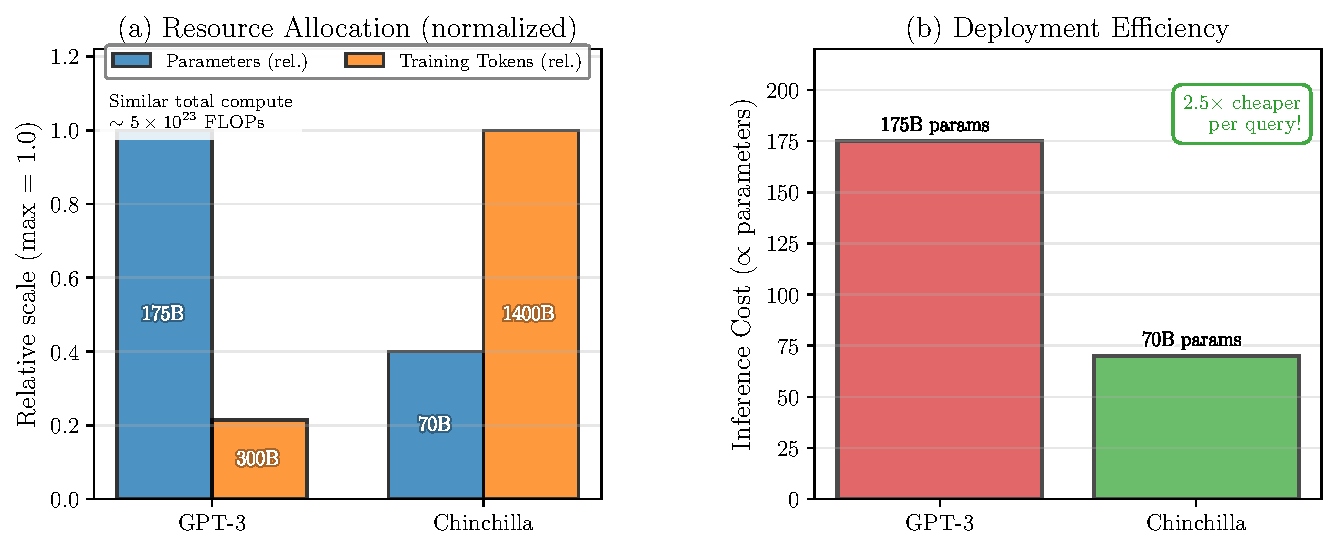
\includegraphics[width=\linewidth]{code/figures/ch12_uncertainty/fig_12_1_chinchilla_vs_gpt3.pdf}
\caption{Chinchilla rebalanced compute budgets: fewer parameters but far more data yielded better accuracy at lower inference cost than GPT-3.}
\label{fig:chinchilla_vs_gpt3}
\end{figure}



\vspace{0.5em}

\textbf{GPT-3:} 175B parameters, 300B tokens, $\sim$3$\times$ compute per token

\textbf{Chinchilla:} 70B parameters, 1.4T tokens, $\sim$0.7$\times$ compute per token (but 4.7$\times$ more tokens)

\vspace{0.5em}

The key insight is that parameters and data are not independent resources. They interact through the compute budget. For a fixed amount of compute $C$, you can train a large model on little data or a small model on lots of data. Chinchilla showed that previous models had chosen the wrong point on this tradeoff curve.

Why does this matter for deployment? Inference cost is proportional to model size, not training data size. A 70B parameter model is much cheaper to run than a 175B parameter model, roughly 2.5$\times$ cheaper in terms of FLOPs per forward pass and memory footprint. If you serve billions of queries, this difference adds up to millions of dollars per year in infrastructure costs.

The Chinchilla discovery crystallized a principle: for a given compute budget $C$, there is an optimal pair $(N^*, D^*)$ of model size $N$ (parameters) and dataset size $D$ (tokens) that minimizes loss. Deviating from this optimal allocation, by making the model too large or training on too little data, wastes resources.

\vspace{1em}

\subsection{Power Laws: The Empirical Regularities}

The Chinchilla paper did more than show one optimal allocation. It revealed the mathematical structure underlying scaling. When researchers plotted loss against compute, parameters, and data across dozens of models spanning several orders of magnitude, they found power law relationships.

A power law is a relationship of the form $y = a x^{-b}$ where $a$ and $b$ are constants. On a log-log plot, power laws appear as straight lines. The exponent $b$ determines how quickly $y$ decreases as $x$ increases; it is the slope on the log-log plot.

Here are the three fundamental scaling laws discovered empirically \citep{kaplan2020scaling,hoffmann2022chinchilla}:

\textbf{Loss versus compute:}
\begin{equation}
L(C) = \left(\frac{C}{C_0}\right)^{-\alpha} + L_{\infty}
\end{equation}

For language models, $\alpha \approx 0.05$ to $0.07$ \citep{kaplan2020scaling,hoffmann2022chinchilla}. This means that every 10$\times$ increase in compute reduces loss by roughly 10 to 15 percent. The term $L_{\infty}$ is an irreducible loss floor; even with infinite compute, there is entropy in natural language that cannot be eliminated.

\textbf{Loss versus parameters:}
\begin{equation}
L(N) = \left(\frac{N}{N_0}\right)^{-\beta} + L_{\infty}
\end{equation}

For language models, $\beta \approx 0.076$ \citep{kaplan2020scaling,hoffmann2022chinchilla}. This means parameters buy you bits of capacity with diminishing returns: the 100th billion parameters help less than the first billion.

\textbf{Loss versus data:}
\begin{equation}
L(D) = \left(\frac{D}{D_0}\right)^{-\gamma} + L_{\infty}
\end{equation}

For language models, $\gamma \approx 0.095$ \citep{kaplan2020scaling,hoffmann2022chinchilla}. Data also exhibits diminishing returns, but slightly less steep than parameters for the regimes studied.

These are not three independent laws. They are different slices of the same constraint: training compute couples parameters and data.

For dense transformer training, a widely used back-of-the-envelope is:
\begin{equation}
C \approx 6ND
\end{equation}

where $N$ is the number of parameters and $D$ is the total number of training tokens \emph{processed} (counting repeats/epochs). The constant 6 is a rough efficiency factor that folds together forward+backward, attention/MLP overhead, and implementation details; different architectures and kernels move it, but the linear dependence on $N$ and $D$ is the key \citep{hoffmann2022chinchilla}.

This constraint creates a tradeoff surface. For fixed $C$, you can choose $(N, D)$ pairs along the curve $C = 6ND$. The optimal pair is the one that minimizes loss $L(N, D)$.

\vspace{1.5em}

\begin{examplebox}
\textbf{Computing the Chinchilla-Optimal Allocation}

\vspace{0.5em}

Suppose you have a compute budget of $C = 10^{23}$ FLOPs. What is the optimal allocation between parameters and data?

\vspace{0.5em}

The Chinchilla paper fit a compute-optimal frontier of the form:
\begin{equation}
N_{\text{opt}} \approx 0.73 \cdot C_{20}^{0.49}, \quad D_{\text{opt}} \approx 22.8 \cdot C_{20}^{0.51}
\end{equation}

where $C_{20} = C / 10^{20}$ measures compute in units of $10^{20}$ FLOPs (about a petaFLOP-day), $N_{\text{opt}}$ is in billions of parameters, and $D_{\text{opt}}$ is in billions of tokens \citep{hoffmann2022chinchilla}. The key qualitative point is that both scale close to $\sqrt{C}$: you should grow model size and data size together as compute increases.

\vspace{0.5em}

For $C = 10^{23}$ FLOPs, we have $C_{20} = 1000$, so the fit gives approximately:
\begin{align}
N_{\text{opt}} &\approx 22 \text{ billion parameters} \\
D_{\text{opt}} &\approx 770 \text{ billion tokens}
\end{align}

On this frontier, the ratio $D/N$ is typically in the \emph{tens} of tokens per parameter (Chinchilla itself is about 20 in this regime); the ratio drifts slowly with compute and depends on the empirical fit.

\vspace{0.5em}

If you instead trained a 100B parameter model (like GPT-3 scale) on the same compute budget, you would only afford $10^{23} / (6 \times 10^{11}) \approx 167$ billion tokens, several times fewer than the compute-optimal data. Your loss would be higher than the compute-optimal point.

\vspace{0.5em}

Conversely, if you trained a 5B parameter model, you could afford $10^{23} / (6 \times 5 \times 10^9) \approx 3.3$ trillion tokens. But you would be over-training: the model does not have enough capacity to benefit from all that data, and you would waste compute on redundant gradient updates.

\vspace{0.5em}

The Chinchilla-optimal allocation minimizes loss by balancing model capacity against data information content.
\end{examplebox}

\begin{figure}[t]
\centering
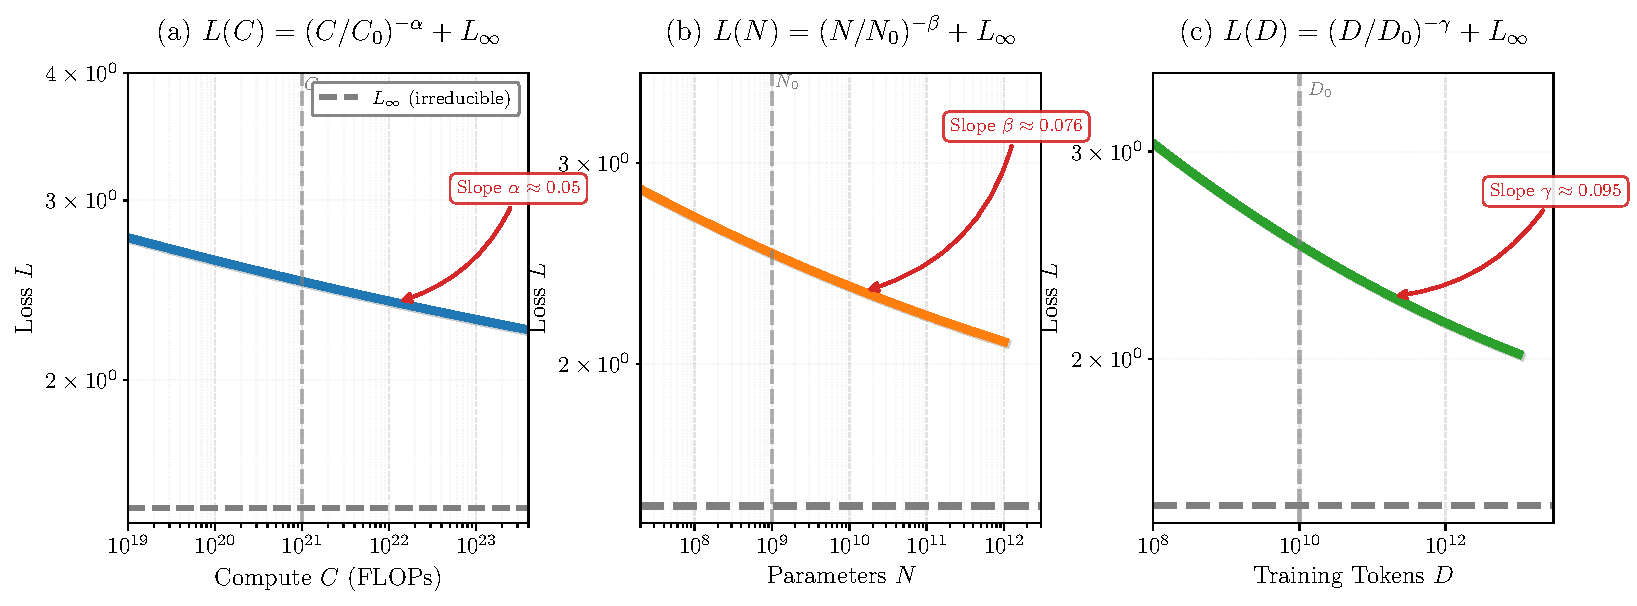
\includegraphics[width=\linewidth]{code/figures/ch12_uncertainty/fig_12_2_scaling_laws.pdf}
\caption{Loss vs. compute, parameters, and data follow power laws; the shallow slopes encode the diminishing returns that define the scaling frontier.}
\label{fig:scaling_laws}
\end{figure}

\begin{figure}[t]
\centering
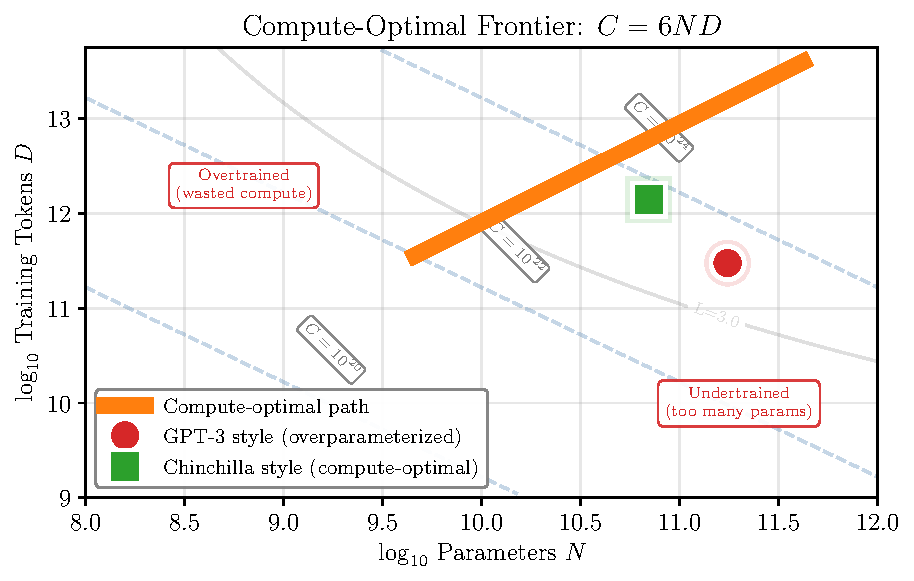
\includegraphics[width=\linewidth]{code/figures/ch12_uncertainty/fig_12_3_compute_optimal_frontier.pdf}
\caption{Compute-optimal training traces a frontier where tokens per parameter stay roughly constant (often tens of tokens per parameter); drifting left or right wastes compute on undertrained weights or unused data.}
\label{fig:compute_optimal_frontier}
\end{figure}


\vspace{1.5em}



\subsection{Information-Theoretic Interpretation}

Why do these power laws exist? The answer lies in rate-distortion theory from Chapter 1 and the compression-generalization connection from Chapter 9. Let me build the intuition step by step.

Think of a language model as a lossy compressor. It takes a sequence of tokens (data) and compresses it into a sequence of predictions (model outputs). The loss measures the quality of this compression: lower loss means better compression, which means the model has captured more structure.

Parameters give the model memory capacity. A larger model can store more information about the training distribution. But this capacity has diminishing returns. The first billion parameters let you capture basic syntax and common word associations. The second billion let you capture more nuanced patterns. The tenth billion let you distinguish rare idioms and complex dependencies. Each additional parameter buys you less marginal information capacity.

From rate-distortion theory, we know that the relationship between rate (bits of information) and distortion (prediction error) follows a power law for many natural sources. The exponent of the power law depends on the intrinsic dimensionality and smoothness of the source. For language, empirical measurements suggest an effective dimensionality that gives the observed exponent $\beta \approx 0.076$.

Data gives the model information content. More tokens mean more examples of the patterns you want to compress. But data also has diminishing returns. The first million tokens teach you basic language structure. The next million refine your estimates. The billionth token fills in rare edge cases. The information content of natural language has structure (it is not uniformly random), so later data provides less new information than early data.

Compute is the resource you spend to match capacity to content. Training is an optimization process that adjusts parameters to minimize loss on data. This process has computational cost proportional to the number of parameters times the number of tokens times the number of training epochs. When you fix the compute budget, you are constraining the product $N \times D$.

The optimal allocation balances capacity and content. If you have too much capacity relative to content ($N$ too large relative to $D$), the model has more parameters than it can effectively train; you are wasting capacity on undertrained weights. If you have too little capacity relative to content ($N$ too small relative to $D$), the model cannot absorb all the information in the data; you are wasting data on a model that cannot learn from it.

The power law exponents $\alpha$, $\beta$, and $\gamma$ encode the rate at which these diminishing returns set in. They are not universal constants; they depend on the data distribution, model architecture, and task. But within a regime (e.g., autoregressive language modeling on internet text with transformer architectures), they are remarkably stable across several orders of magnitude.

\vspace{1em}

\begin{geometrylens}
\textbf{Scaling Laws as Rate-Distortion Curves}

\vspace{0.5em}

Rate-distortion theory tells us that there is a fundamental tradeoff between the rate $R$ (information capacity) and distortion $D$ (prediction error). For smooth sources, this tradeoff often follows a power law: $D \propto R^{-\alpha}$.

\vspace{0.5em}

In language models, the "rate" is determined by model size $N$ (memory capacity) and data size $D$ (information content). The compute budget $C$ constrains how much rate you can achieve: $R \propto \sqrt{C}$ when optimally allocated.

\vspace{0.5em}

The scaling law $L(C) \propto C^{-\alpha}$ is exactly the rate-distortion curve: as you increase information capacity (via compute), distortion (loss) decreases with diminishing returns. The exponent $\alpha$ encodes the intrinsic difficulty of compressing the source.

\vspace{0.5em}

Geometrically, the space of models is a manifold parameterized by $(N, D)$. The loss function defines a scalar field on this manifold. Scaling laws describe the gradient of this field: how loss changes as you move through model space. The Chinchilla-optimal path is the trajectory through this space that descends the loss gradient most efficiently given the compute constraint (Figure~\ref{fig:compute_optimal_frontier}).
\end{geometrylens}

\vspace{1.5em}

\subsection{Emergent Abilities and Phase Transitions}

Scaling laws describe smooth changes in loss, but some benchmark curves look \emph{phase-transition-like}: a capability is hard to detect at small scale and then becomes reliable over a relatively narrow range of model sizes. These are often called emergent abilities \citep{wei2022emergent}. The word "emergent" is controversial; some apparent jumps are artifacts of metric choice and thresholding \citep{schaeffer2023emergentmirage}, but the practical lesson is real: some tasks feel impossible until you cross a capacity-and-data threshold.

\begin{figure}[t]
\centering
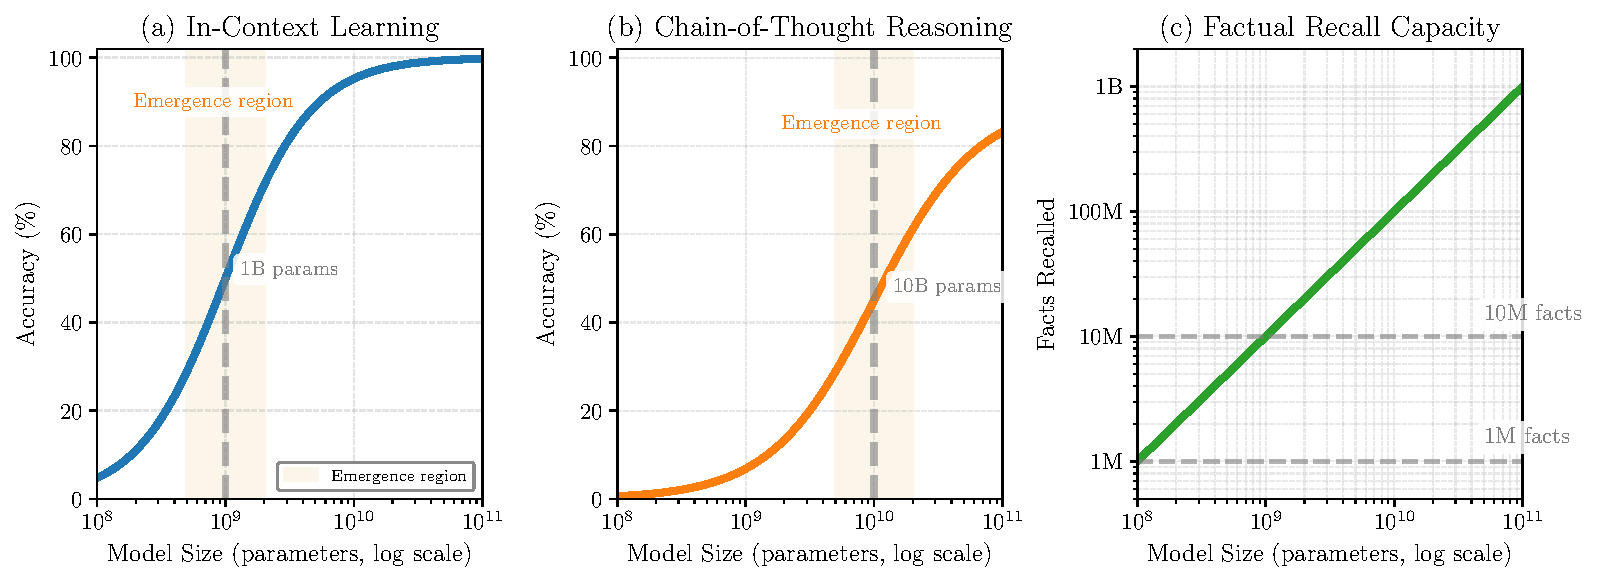
\includegraphics[width=\linewidth]{code/figures/ch12_uncertainty/fig_12_4_emergent_abilities.pdf}
\caption{Schematic: some benchmark curves look thresholded; below a region performance is near chance, and above it it can rise rapidly over a narrow range of scales.}
\label{fig:emergent_abilities}
\end{figure}



\textbf{In-context learning} is the ability to improve from examples provided in the prompt without any gradient updates. On many few-shot benchmarks, models below $\sim$1B parameters show weak gains, while models in the multi-billion to tens-of-billions range often show clear few-shot improvements. The transition can look sharp on thresholded metrics.

\textbf{Chain-of-thought reasoning} is the ability to solve complex problems by generating intermediate reasoning steps. Across tasks, it often becomes useful somewhere in the $\sim$10B to $\sim$100B range, but the location depends strongly on prompting, evaluation, and training data. Smaller models can generate reasoning-like text without reliable correctness; larger models are more likely to use intermediate steps to reach the right answer.

\textbf{Few-shot instruction following} is the ability to follow new instructions after seeing only a few examples. This tends to be more gradual, and it is heavily influenced by data curation and alignment training: the same base model can look non-instruction-following before instruction-tuning and competent after it.

Why do these abilities emerge suddenly instead of scaling smoothly? One explanation is that they are not truly discontinuous; they are smooth in the right metric, but that metric is not cross entropy loss. Cross entropy measures average per-token prediction quality, which improves smoothly with scale. But solving a math problem correctly requires getting every step right, which has a sharp threshold: below some loss level, you make too many errors to reach the right answer; above it, you succeed reliably.

From an information-theoretic perspective, these shifts are consistent with crossing capacity thresholds. Certain tasks require a minimum amount of information capacity \emph{and} the right training signal to perform non-trivially. Below that region, performance is dominated by errors. Above it, the same smooth improvement in per-token loss can translate into a large jump in end-task success rate.

These thresholds are task-dependent and architecture-dependent. Algorithmic improvements can lower the capacity threshold for a given capability. But for any fixed architecture and task, there will be some minimum scale below which the capability is absent and above which it is present.

\vspace{1.5em}

\begin{examplebox}
\textbf{Predicting Emergence from Information Requirements}

\vspace{0.5em}

Consider the task of recalling a specific fact from memory (e.g., "In what year did the Battle of Waterloo occur?"). The model needs to have encoded this fact during training and retrieve it at test time.

\vspace{0.5em}

As a cartoon, imagine a fact is answered by a single token chosen from a vocabulary of size $V$. Identifying that token takes about $\log_2 V$ bits. For a vocabulary of 50,000, $\log_2 V \approx 15.6$ bits per fact.

\vspace{0.5em}

A model with $N$ parameters, where each parameter is stored with $b$ bits of precision, has roughly $Nb$ bits of total capacity. But not all of this capacity is available for fact storage; much of it encodes linguistic patterns, grammar, and common sense reasoning.

\vspace{0.5em}

Let $f$ be the fraction of parameter capacity that ends up usable for factual recall (the rest supports syntax, generalization, and shared features). Then a back-of-the-envelope estimate is:
\begin{equation}
\text{Facts} \approx \frac{f \, N \, b}{\log_2 V}
\end{equation}

\vspace{0.5em}

For a 1B parameter model with 16-bit precision and a conservative $f = 0.01$:
\begin{equation}
\text{Facts} \approx \frac{0.01 \times 10^9 \times 16}{15.6} \approx 10 \text{ million}
\end{equation}

\vspace{0.5em}

This is not a literal memory-size calculation; parameters are shared, continuous, and trained by gradient descent. The point is that as $N$ grows, factual recall capacity grows, and tasks with hard thresholds can appear to "switch on" once you have enough stored knowledge to clear the bar.

\vspace{0.5em}

The "emergence" of factual recall is not truly discontinuous. It is smooth in the number of facts recalled, but tasks often have hard thresholds (e.g., you either know enough geography to pass a test or you do not), creating apparent discontinuities.
\end{examplebox}

\vspace{1.5em}

\subsection{When to Scale Versus When to Stop}

Scaling laws give you predictive power, but how do you use them to make decisions? The answer depends on your constraints and objectives. Let me walk through a decision framework.

\textbf{Step 1: Define your loss target.} What level of performance do you need? This might be specified as cross entropy loss, accuracy on a benchmark, or task-specific metrics. If you do not have a hard target, use scaling laws to understand the performance frontier and decide what is achievable.

\textbf{Step 2: Estimate your compute budget.} How much can you spend on training? This includes GPU-hours, electricity, and time. Convert this to FLOPs using the effective throughput of your hardware setup (roughly $10^{17}$ to $10^{18}$ FLOPs per GPU-hour for A100-class accelerators; the exact number depends on utilization and precision).

\textbf{Step 3: Use scaling laws to find the optimal $(N, D)$ allocation.} Apply the Chinchilla formula: $N_{\text{opt}} \propto C^{0.5}$ and $D_{\text{opt}} \propto C^{0.5}$. This gives you a starting point for model size and data size.

\textbf{Step 4: Adjust for your deployment constraints.} If inference cost is critical (high query volume, latency-sensitive), bias toward smaller $N$ and larger $D$. You can afford to spend more compute on training if it saves on inference. If training budget is very limited but inference budget is generous, bias toward larger $N$ and accept slightly higher loss.

\textbf{Step 5: Adjust for task-specific considerations.} If your task benefits heavily from in-context learning or few-shot adaptation, you need at least 10B parameters even if compute-optimal would suggest smaller. If you are fine-tuning from a pretrained model, you can use a smaller $D$ because you start with better initialization.

\textbf{Step 6: Run small-scale experiments to validate.} Scaling laws extrapolate from smaller models to larger ones. Before committing to a massive training run, train models at 1/10th and 1/100th the scale and verify that loss scales as predicted. If your smaller runs deviate from power laws, diagnose the issue before scaling up.

Let me make this concrete with a worked example.

\vspace{1.5em}

\begin{examplebox}
\textbf{Scaling Decision for a Domain-Specific Model}

\vspace{0.5em}

Suppose you want to build a language model for medical text. You have access to 100 billion tokens of medical literature and 10,000 GPU-hours on A100 GPUs (roughly $2 \times 10^{21}$ FLOPs effective).

\vspace{0.5em}

\textbf{Compute-optimal allocation:}

Using $C \approx 2 \times 10^{21}$ (so $C_{20} \approx 20$), the Chinchilla formula suggests:
\begin{align}
N_{\text{opt}} &\approx 3 \text{ billion parameters} \\
D_{\text{opt}} &\approx 100 \text{ billion tokens}
\end{align}

You have 100B tokens available, which is right around the compute-optimal frontier. This suggests you are roughly balanced: your main choice is whether to tilt toward lower inference cost (smaller $N$) or higher peak capability (larger $N$).

\vspace{0.5em}

\textbf{Adjustment for domain:}

Medical language has specialized terminology and concepts. You might benefit from a larger model even if it means training on a bit less data, because the additional capacity helps capture domain-specific patterns. Consider training a 5B parameter model on 70B tokens (still within your compute budget).

\vspace{0.5em}

\textbf{Adjustment for deployment:}

You plan to deploy this model in a hospital setting with limited GPU access. Inference latency is critical. This biases you toward a smaller model. Stick closer to the compute-optimal 3B parameters (or smaller).

\vspace{0.5em}

\textbf{Fine-tuning strategy:}

Instead of training from scratch, consider starting from a pretrained general-purpose model (e.g., a 7B parameter model trained on web text). Fine-tune on 50B tokens of medical text. This uses your compute budget to specialize an already-capable model, often achieving better performance than training a smaller model from scratch.

\vspace{0.5em}

\textbf{Final decision:}

Fine-tune a pretrained 3B parameter model on 50B tokens of high-quality medical text. This balances domain specificity, inference cost, and compute efficiency. Validate with a small pilot: fine-tune a 300M parameter model on 5B tokens (1/10th scale) and verify the loss scales as expected before committing to the full run.
\end{examplebox}

\vspace{1.5em}

\vspace{2em}

%==========================
\section{Training Dynamics in Practice}
%==========================

Scaling laws tell you what performance to expect at different scales, but they do not tell you how to actually train models reliably. Training large models is a complex engineering challenge with many failure modes. This section covers the practical dynamics of training: learning rates, batch sizes, stability, and distributed training.

\vspace{1em}

\subsection{Learning Rate Schedules}

The learning rate is the most important hyperparameter in training. Set it too high and your loss explodes. Set it too low and training is inefficient. Worse, the optimal learning rate changes during training, so you need a schedule that adapts over time.

The standard approach uses three phases: warmup, stable training, and decay.

\textbf{Warmup} means starting with a very small learning rate and gradually increasing it over the first few thousand steps. Why is this necessary? Early in training, the loss landscape is poorly explored. The model is at a random initialization, and the curvature (Hessian) at this point might be very different from the curvature at the eventual optimum. If you start with a large learning rate, you risk overshooting and destabilizing the optimization.

During warmup, the optimizer explores the local geometry and adjusts to the scale of the gradients. A typical warmup schedule increases the learning rate linearly from a small value (e.g., $10^{-7}$) to the target value (e.g., $3 \times 10^{-4}$) over a few thousand steps.

\begin{figure}[t]
\centering
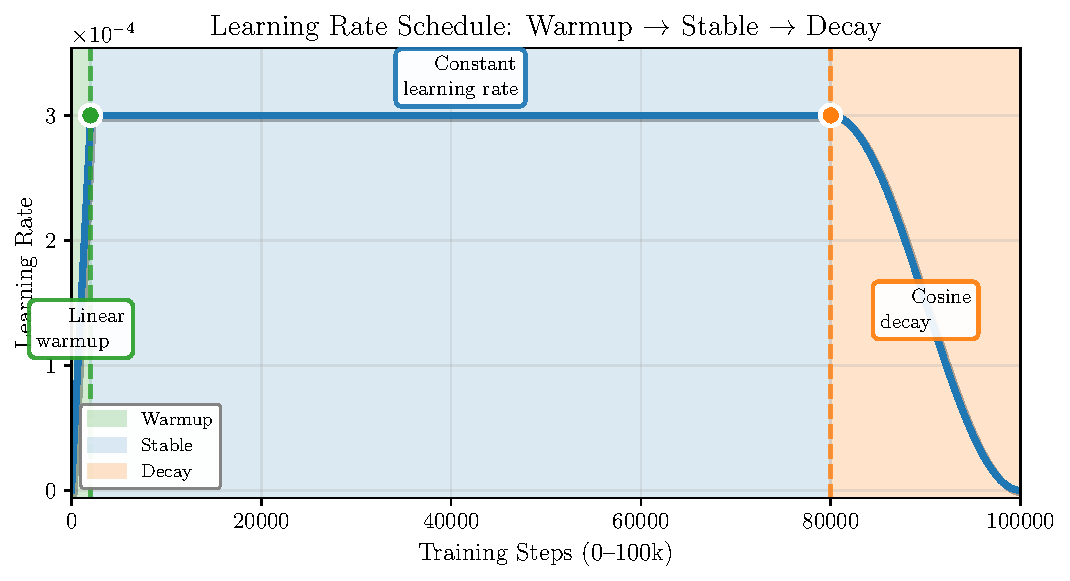
\includegraphics[width=\linewidth]{code/figures/ch12_uncertainty/fig_12_5_learning_rate_schedule.pdf}
\caption{Learning-rate schedules combine warmup, a flat plateau, and decay; tuning their shape is critical for stable, efficient training at scale.}
\label{fig:learning_rate_schedule}
\end{figure}



Warmup length is an empirical knob. A common heuristic is to warm up for a fixed \emph{amount of data} (tokens) or a fixed fraction of total training, so if you increase batch size you can usually shorten warmup in steps. The goal is simple: by the end of warmup, optimizer statistics and activations have stabilized enough that the peak learning rate is safe.

\textbf{Stable training} is the main phase where most learning happens. You hold the learning rate constant or decrease it slowly. For language models, learning rates typically range from $10^{-4}$ to $10^{-3}$ depending on model size and batch size. Larger models often need smaller learning rates because the loss landscape has more parameters and more directions to balance.

\textbf{Decay} means gradually reducing the learning rate toward the end of training. This helps the optimizer settle into a minimum rather than bouncing around it. Two common decay schedules are:

Cosine decay: $\eta(t) = \eta_{\text{max}} \cdot \frac{1 + \cos(\pi t / T)}{2}$ where $t$ is the current step and $T$ is the total number of training steps. This smoothly decreases the learning rate to zero following a cosine curve.

Linear decay: $\eta(t) = \eta_{\text{max}} \cdot (1 - t/T)$. This decreases linearly to zero.

Cosine decay is more popular in practice because it spends more time at higher learning rates (which accelerates training) and only decreases sharply at the very end.

The relationship between learning rate and batch size is often summarized by the linear scaling rule: if you multiply the batch size by $k$, you can multiply the learning rate by $k$ as well, at least up to a critical batch size \citep{goyal2017imagenet}. This rule comes from the observation that larger batches give more accurate gradient estimates, so you can take larger steps without overshooting.

However, the linear scaling rule breaks down at large batch sizes. Empirically, there is a critical batch size beyond which further increases do not allow higher learning rates and do not reduce the number of optimization steps much further \citep{mccandlish2018batch}. This critical batch size is task- and model-dependent, but it typically ranges from 1,024 to 32,768 for language models.

\vspace{1.5em}

\begin{examplebox}
\textbf{Designing a Learning Rate Schedule}

\vspace{0.5em}

Suppose you are training a 1B parameter language model for 100,000 steps with a batch size of 512.

\vspace{0.5em}

\textbf{Warmup:} Linear warmup from $10^{-7}$ to $3 \times 10^{-4}$ over 2,000 steps. This gives the optimizer time to explore the initial landscape.

\vspace{0.5em}

\textbf{Stable training:} Hold at $3 \times 10^{-4}$ from step 2,000 to step 80,000. This is where most learning happens.

\vspace{0.5em}

\textbf{Cosine decay:} From step 80,000 to step 100,000, apply cosine decay:
\begin{equation}
\eta(t) = 3 \times 10^{-4} \cdot \frac{1 + \cos(\pi (t - 80000) / 20000)}{2}
\end{equation}

At step 80,000, $\eta = 3 \times 10^{-4}$. At step 100,000, $\eta = 0$.

\vspace{0.5em}

\textbf{Batch size experiment:}

If you double the batch size to 1,024, you can double the peak learning rate to $6 \times 10^{-4}$ (by the linear scaling rule) and train for 50,000 steps (half as many because each step processes twice as much data). The warmup can be shortened to 1,000 steps because the gradients are lower-variance.

\vspace{0.5em}

\textbf{Critical batch size:}

If you increase the batch size to 16,384 (32× larger), the linear scaling rule suggests a learning rate of $32 \times 3 \times 10^{-4} \approx 10^{-2}$. But this is likely above the critical batch size for stability. Empirically, you would find that learning rates above $3 \times 10^{-3}$ cause instability, even with the larger batch. You hit the critical batch size and cannot scale further.
\end{examplebox}

\vspace{1.5em}

\subsection{Batch Size and Parallelism}

Batch size determines how many examples you process before updating the model's parameters. It is a tradeoff between gradient variance and computational efficiency.

\textbf{Small batches} (32 to 256 examples) give noisy gradient estimates.

\begin{figure}[t]
\centering
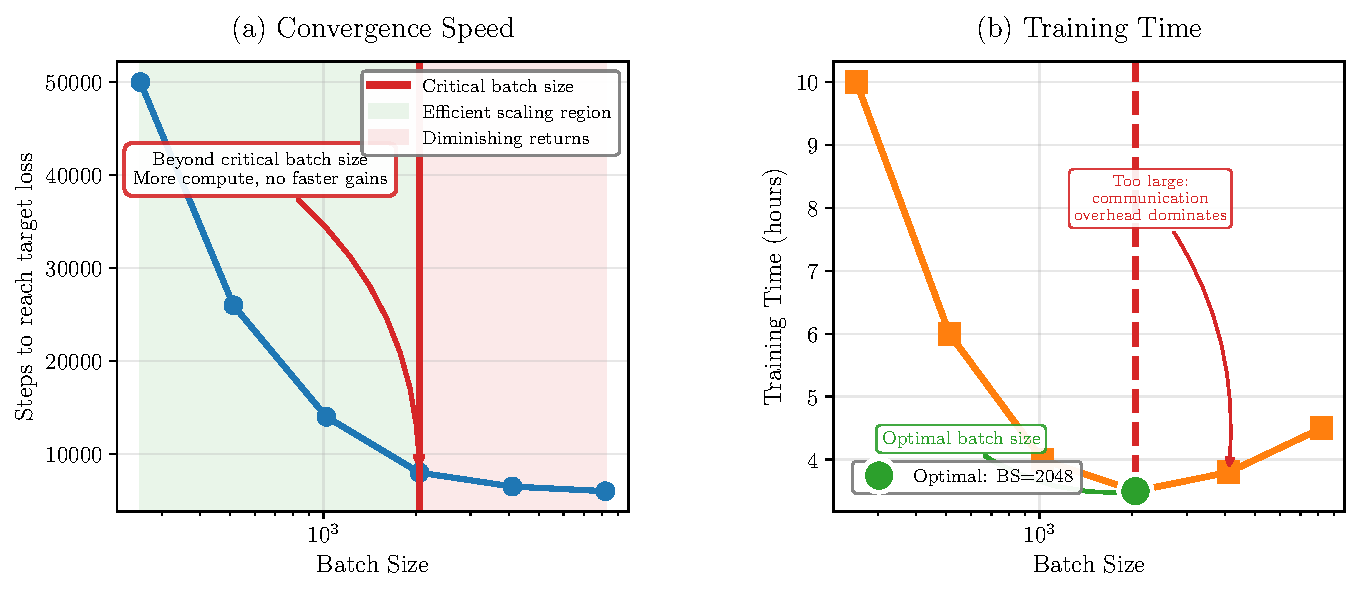
\includegraphics[width=\linewidth]{code/figures/ch12_uncertainty/fig_12_6_critical_batch_size.pdf}
\caption{Critical batch size marks where larger batches stop buying faster convergence; linear learning-rate scaling fails beyond this elbow.}
\label{fig:critical_batch_size}
\end{figure}

This noise acts as implicit regularization, helping the optimizer explore the loss landscape and avoid sharp minima (recall the discussion of flatness from Chapter 9). Small batches also allow faster iteration: you update parameters more frequently, which can accelerate convergence in terms of wall-clock time if you are not compute-limited.


\textbf{Large batches} (1,024 to 32,768 examples) give more accurate gradient estimates. This reduces variance and makes optimization more stable. Large batches also improve hardware utilization: modern GPUs parallelize matrix operations, and larger batches mean larger matrices, which use the hardware more efficiently.

The tradeoff is between exploration and efficiency. Small batches explore more but underutilize hardware. Large batches utilize hardware efficiently but can converge to worse solutions if the batch size exceeds the critical threshold.

The \textbf{critical batch size} is the point where increasing the batch size no longer improves convergence speed (in terms of the number of steps needed to reach a target loss). Beyond this size, larger batches only increase per-step cost without reducing the total number of steps. For language models, the critical batch size is typically between 0.1 and 1 million tokens (batch size times sequence length).

In practice, you often want to use batches larger than what fits in GPU memory. The solution is \textbf{gradient accumulation}: split the batch across multiple forward-backward passes, accumulate the gradients, and then update the parameters once after all sub-batches have been processed. This gives you the benefit of large batch training without exceeding memory constraints.

For example, if your GPU can fit a batch of 16 examples but you want an effective batch of 512, you run 32 forward-backward passes with a batch of 16, accumulate the gradients, and then update. From the optimizer's perspective, this is equivalent to processing all 512 examples at once.

\vspace{1em}

\subsection{Stability and Recovery}

Training large models is fragile. Loss can spike unexpectedly, gradients can explode or vanish, and numerical precision issues can cause NaNs (not-a-number values) to propagate through the model. Robust training requires monitoring for these issues and recovering gracefully when they occur.

\begin{figure}[t]
\centering
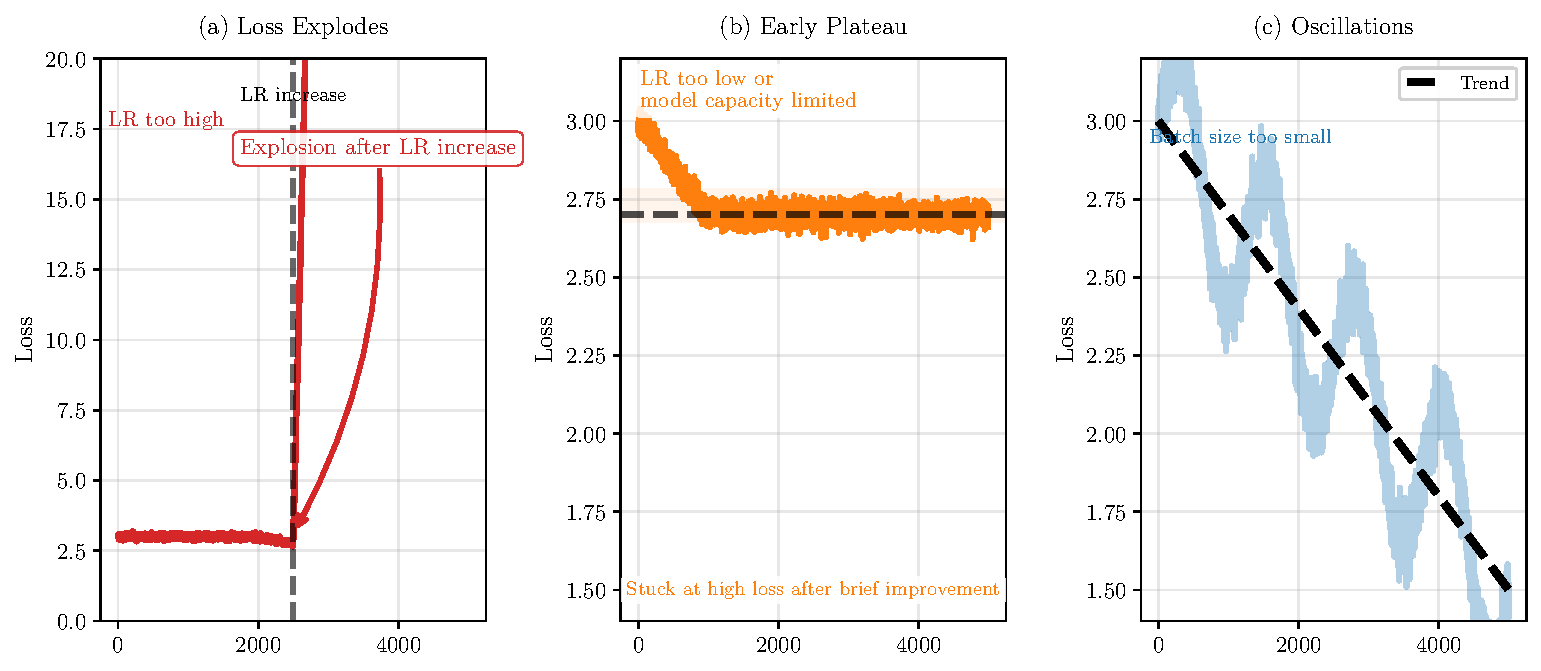
\includegraphics[width=\linewidth]{code/figures/ch12_uncertainty/fig_12_7a_training_instabilities.pdf}
\caption{Training instabilities: loss spikes, exploding gradients, and NaNs. Monitor early and recover quickly to avoid wasted compute.}
\label{fig:training_instabilities}
\end{figure}

\begin{figure}[t]
\centering
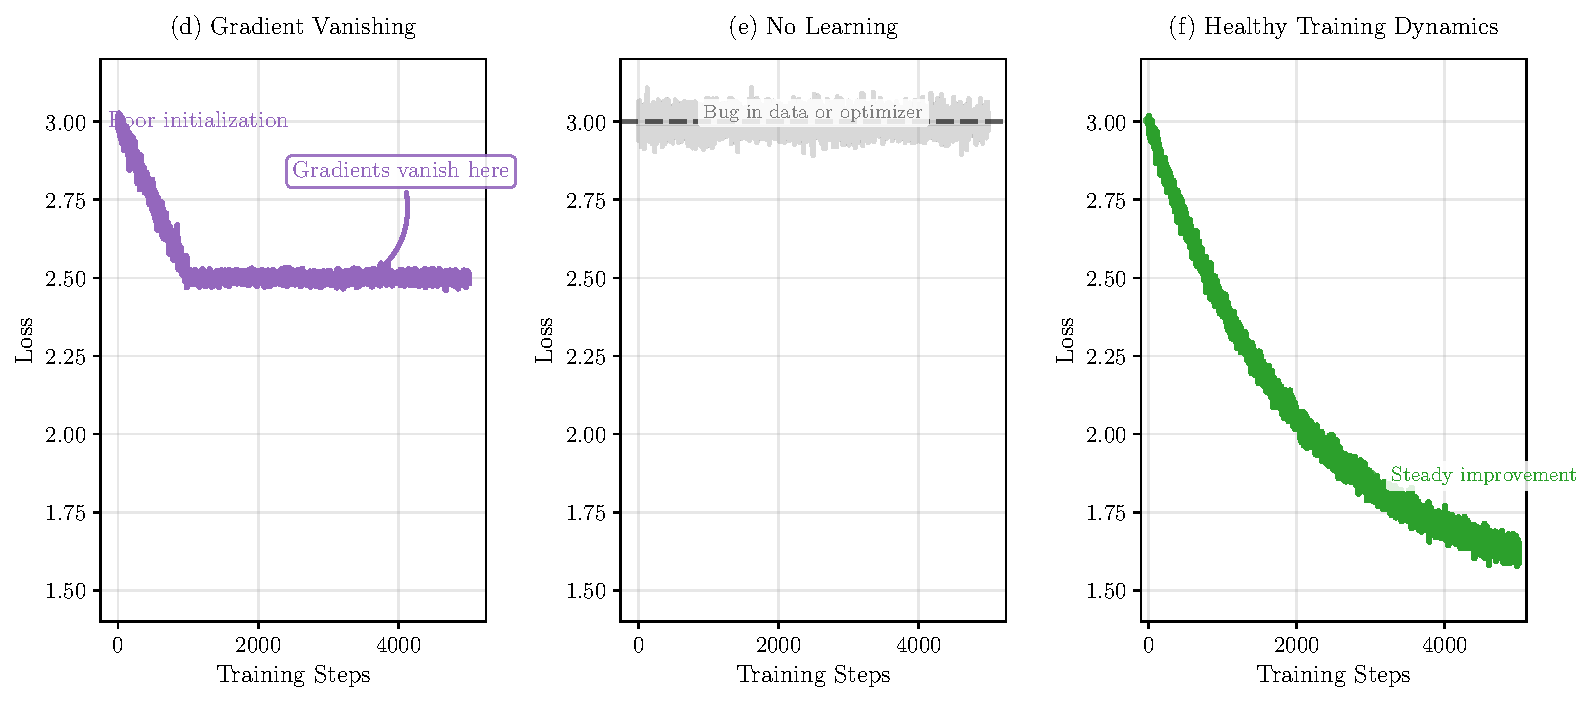
\includegraphics[width=\linewidth]{code/figures/ch12_uncertainty/fig_12_7b_learning_failures.pdf}
\caption{Learning failures and diagnosis patterns: vanishing/exploding gradients, dead activations, and optimizer issues; use a systematic debugging checklist.}
\label{fig:learning_failures}
\end{figure}



\textbf{Loss spikes} are sudden increases in loss during training. They have several common causes:

\begin{itemize}
\item Learning rate too high: The optimizer takes a step that overshoots a minimum and lands in a high-loss region. The solution is to reduce the learning rate or improve the learning rate schedule.

\item Batch statistics: A single bad batch (e.g., very long sequences or rare tokens) can produce abnormally large gradients. The solution is to use gradient clipping or increase batch size to reduce variance.

\item Numerical instability: Intermediate activations grow very large or very small, causing overflow or underflow. The solution is to use mixed precision training with careful scaling or switch to a more stable architecture (e.g., Pre-LN instead of Post-LN).
\end{itemize}

When a loss spike occurs, the standard recovery strategy is to roll back to a recent checkpoint (typically saved every few thousand steps) and resume training with a reduced learning rate. Some training frameworks implement automatic recovery: they detect spikes, revert to the last stable checkpoint, and reduce the learning rate by a factor of 2 or 5.

\textbf{Gradient clipping} is a simple but effective technique to prevent exploding gradients. Before applying a gradient update, you compute the global norm of the gradient (the L2 norm across all parameters). If this norm exceeds a threshold (commonly 1.0), you scale the gradient down to have norm equal to the threshold. This prevents any single update from being too large, at the cost of slightly biasing the gradient direction.

The clipping threshold should be chosen based on the typical gradient norm during stable training. If you clip too aggressively (threshold too small), you slow down training by limiting step size. If you clip too loosely (threshold too large), you do not prevent spikes. A good heuristic is to set the threshold to 2× the median gradient norm observed during the first few thousand steps.

\textbf{NaN detection} is critical because NaNs propagate: once a single activation or gradient becomes NaN, all subsequent computations will also be NaN, and the model is unrecoverable without rollback. Modern training frameworks include NaN detection: if any parameter, gradient, or loss becomes NaN, the framework immediately halts training, prints diagnostic information, and optionally reverts to a checkpoint.

To prevent NaNs in the first place, use mixed precision training with loss scaling \citep{micikevicius2018mixedprecision}. Mixed precision uses 16-bit floats (half precision) for most computations to save memory and increase throughput, but accumulates gradients in 32-bit precision to avoid numerical errors. Loss scaling multiplies the loss by a large constant before backpropagation, which shifts the gradient values into a range where half precision can represent them accurately. After clipping and before updating parameters, you divide by the same constant to recover the true gradient scale.

\textbf{Checkpoint frequency} is a tradeoff between recovery cost and storage cost. Saving checkpoints more frequently reduces the amount of lost progress when you need to roll back, but it consumes more disk space and I/O bandwidth. A typical strategy is to save every 1,000 to 5,000 steps, keeping the last 3 to 5 checkpoints. For very long training runs (weeks or months), you might also save milestone checkpoints at specific intervals (e.g., every 10,000 steps) that you keep permanently for later analysis.

\vspace{1.5em}

\begin{examplebox}
\textbf{Diagnosing and Recovering from a Loss Spike}

\vspace{0.5em}

You are training a 7B parameter model. At step 45,000, the loss suddenly jumps from 2.3 to 6.8 in a single step. The training log shows:

\vspace{0.3em}

\begin{verbatim}
Step 44999: loss=2.31, grad_norm=0.42, lr=3e-4
Step 45000: loss=6.83, grad_norm=24.7, lr=3e-4
Step 45001: loss=NaN, grad_norm=NaN, lr=3e-4
\end{verbatim}

\vspace{0.5em}

\textbf{Diagnosis:} The gradient norm at step 45,000 is 24.7, far larger than the typical value of 0.4. This suggests a bad batch or numerical instability. The spike caused the loss to increase dramatically, and by step 45,001, NaNs have appeared.

\vspace{0.5em}

\textbf{Recovery:}

1. Revert to the checkpoint at step 44,000 (the last saved checkpoint before the spike).

2. Resume training with gradient clipping threshold set to 1.0 (was previously unclipped or set too high).

3. Reduce the learning rate by a factor of 2: from $3 \times 10^{-4}$ to $1.5 \times 10^{-4}$.

4. Inspect the batch at step 45,000 to see if there was an anomaly (e.g., an unusually long sequence or a corrupted example). If found, filter it from the training data.

\vspace{0.5em}

\textbf{Prevention for future training:}

Enable automatic gradient clipping from the start with threshold 1.0. Use mixed precision training with dynamic loss scaling to prevent numerical issues. Save checkpoints every 2,000 steps instead of 5,000 to reduce recovery cost.
\end{examplebox}

\vspace{1.5em}

\subsection{Distributed Training Essentials}

Training large models requires multiple GPUs, often hundreds or thousands. Distributed training splits the work across GPUs using one of three main paradigms: data parallelism, model parallelism, or pipeline parallelism. Each paradigm has different tradeoffs and is suited to different model sizes.

\textbf{Data parallelism} splits the batch across GPUs. Each GPU holds a full copy of the model and processes a subset of the batch. After computing gradients locally, GPUs synchronize by averaging their gradients (this is called all-reduce), and then all GPUs update their parameters identically. Data parallelism is the simplest approach and scales efficiently up to batch sizes where the critical batch size is reached.

\begin{figure}[t]
\centering
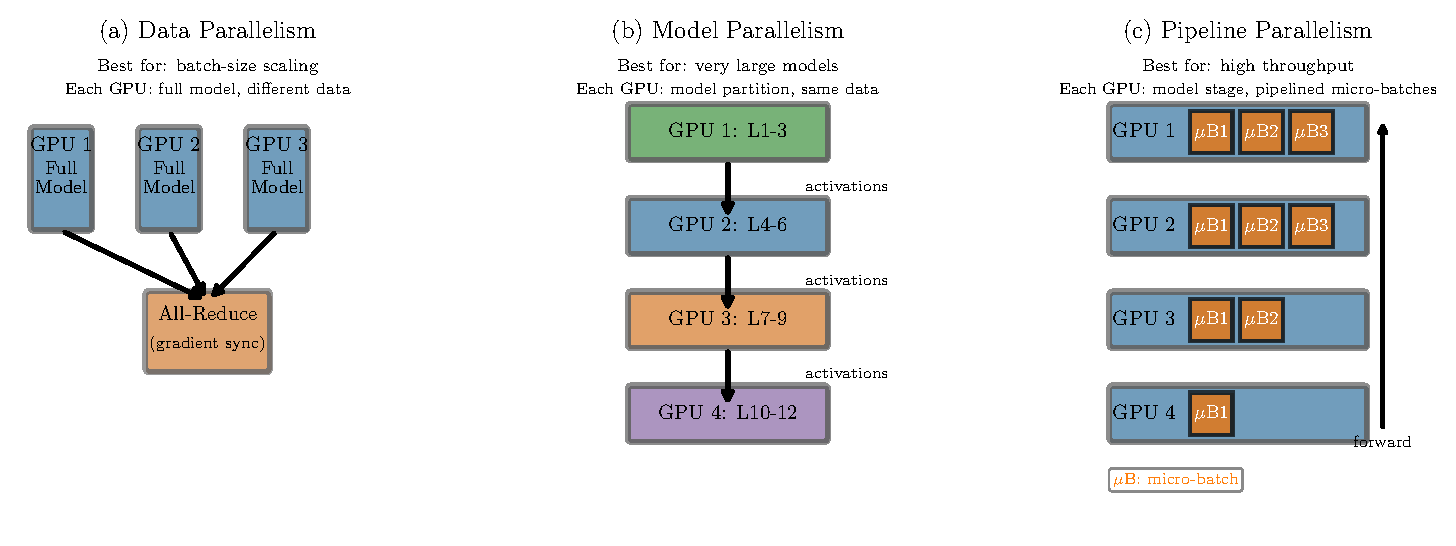
\includegraphics[width=\linewidth]{code/figures/ch12_uncertainty/fig_12_8_distributed_training.pdf}
\caption{Distributed training mixes data, tensor, and pipeline parallelism; the right blend maximizes throughput while respecting memory and bandwidth limits.}
\label{fig:distributed_training}
\end{figure}



The main cost of data parallelism is communication. The all-reduce operation must transfer gradients between all GPUs, which requires bandwidth proportional to the model size. For a 10B parameter model, this is 40 GB per update (assuming 32-bit gradients). If your interconnect bandwidth is 100 GB/s, this takes 0.4 seconds. If your forward-backward pass takes 0.5 seconds, you spend nearly half your time on communication.

To reduce communication cost, use gradient compression (e.g., 16-bit gradients instead of 32-bit) or gradient accumulation (communicate less frequently by accumulating gradients locally over multiple steps). Modern frameworks like PyTorch's DistributedDataParallel (DDP) also overlap computation and communication: while one layer is computing gradients, another layer is communicating its gradients in the background.

\textbf{Model parallelism} splits the model across GPUs. Each GPU holds a subset of the layers or a partition of the weight matrices. This is necessary when the model is too large to fit in a single GPU's memory. The simplest form is tensor parallelism, where you split large matrices (like attention projections) across GPUs. For example, if the attention output has dimension 8,192, you can split it into four chunks of 2,048 and compute each chunk on a different GPU.

Model parallelism introduces communication overhead because activations must be transferred between GPUs. If layer $k$ is on GPU 1 and layer $k+1$ is on GPU 2, the output of layer $k$ must be sent to GPU 2 before layer $k+1$ can run. This creates dependencies that limit parallelism.

Efficient model parallelism requires careful partitioning to minimize communication. For transformers, a common strategy is to parallelize within layers (split attention and feed-forward matrices across GPUs within the same layer) rather than across layers. This keeps most communication within a layer, which happens in parallel, rather than sequentially between layers.

\textbf{Pipeline parallelism} splits the model into stages across GPUs and pipelines the batch through the stages. Each GPU computes one stage of the forward pass, passes the activations to the next GPU, and then computes the backward pass for that stage. Meanwhile, the next GPU is processing the forward pass for the next micro-batch. This creates a pipeline where multiple micro-batches are in flight simultaneously.

Pipeline parallelism improves utilization by overlapping computation across stages. The challenge is the "bubble" at the beginning and end of each batch: the first stage must fill the pipeline before the last stage has work, and the last stage finishes before the first stage starts on the next batch. This bubble reduces efficiency, but it can be minimized by using small micro-batches and many pipeline stages.

The choice between these paradigms depends on model size and hardware:

\begin{itemize}
\item \textbf{Small models} (< 1B parameters): Use data parallelism only. The model fits in a single GPU, and data parallelism scales efficiently.

\item \textbf{Medium models} (1B to 20B parameters): Use data parallelism plus tensor parallelism within nodes. Each node runs tensor parallelism across 8 GPUs to fit the model, and data parallelism across nodes.

\item \textbf{Large models} (20B to 100B+ parameters): Use all three paradigms together. Pipeline parallelism across nodes, tensor parallelism within nodes, and data parallelism across replicas. This is called 3D parallelism.
\end{itemize}

\vspace{1em}

\subsection{When Training Goes Wrong}

Let me give you a taxonomy of failure modes and how to diagnose them. When training goes wrong, the loss curve is your primary diagnostic tool. Different failure modes produce characteristic loss curve patterns.

\textbf{Loss explodes} (increases rapidly after a few steps): Learning rate is too high. The optimizer is taking steps that overshoot minima and land in high-loss regions. Reduce the learning rate by a factor of 2 to 10 and restart. If the explosion happens after many steps of stable training, this might be a numerical instability; enable gradient clipping and mixed precision training.

\textbf{Loss plateaus early} (stops decreasing after reaching a high value): Learning rate is too low. The optimizer is taking tiny steps and gets stuck in a poor local minimum. Increase the learning rate by a factor of 2 to 5. Alternatively, the model might be too small for the task; consider scaling up.

\textbf{Loss oscillates} (increases and decreases repeatedly): Batch size is too small, causing high gradient variance. Increase the batch size or use gradient accumulation. Alternatively, the learning rate might be slightly too high; reduce it by 20 to 50 percent.

\textbf{Gradients vanish} (gradient norms become very small, loss stops improving): Initialization is poor or the architecture has vanishing gradient problems. For poor initialization, use better initialization schemes (e.g., Kaiming initialization for ReLU networks, Xavier initialization for tanh networks). For architecture issues, switch to architectures with residual connections or use gradient clipping to prevent vanishing.

\textbf{Loss does not decrease at all} (stays near the initial value): The model is not learning. Check that data is being read correctly (the data loader is not returning the same batch repeatedly). Check that the optimizer is actually updating parameters (log parameter norms before and after updates). Check that the loss function is correctly implemented. Verify that the learning rate is not so small that progress is imperceptible.

\textbf{Loss decreases then increases} (overfitting): This usually does not happen in large-scale pretraining (you underfit, not overfit), but it can occur in fine-tuning. The model is fitting the training set but not generalizing. Use regularization (weight decay, dropout), early stopping, or increase the training data.

\vspace{1.5em}

\begin{examplebox}
\textbf{Debug Checklist for Training Failures}

\vspace{0.5em}

When training fails, work through this checklist systematically:

\vspace{0.5em}

\textbf{1. Verify the data pipeline:}
\begin{itemize}
\item Print the first batch and inspect it manually. Are the inputs and labels correctly formatted?
\item Check that batches are different. Log batch statistics (mean, variance) across steps.
\item Verify that data augmentation or tokenization is not corrupting examples.
\end{itemize}

\textbf{2. Check the loss function:}
\begin{itemize}
\item Compute the loss on a single batch manually and compare to the reported loss.
\item Verify that the loss makes sense for random predictions (e.g., for classification with $C$ classes, random predictions should give loss $\log C$).
\end{itemize}

\textbf{3. Inspect gradients:}
\begin{itemize}
\item Log gradient norms for each layer. Are some layers getting very large or very small gradients?
\item Check for NaNs or infinities in gradients.
\item Verify that gradients are nonzero (if all gradients are zero, the model is not learning).
\end{itemize}

\textbf{4. Validate the optimizer:}
\begin{itemize}
\item Log parameter norms before and after updates. Are parameters changing?
\item Check that the learning rate is not accidentally set to zero.
\item Verify that weight decay or other regularization is not too strong.
\end{itemize}

\textbf{5. Test on a tiny dataset:}
\begin{itemize}
\item Overfit on a single batch. Can the model achieve zero loss on one batch? If not, there is a bug in the model or loss.
\item If the model can overfit one batch, scale up gradually (10 batches, 100 batches) and verify loss decreases smoothly.
\end{itemize}

\vspace{0.5em}

This checklist catches most training bugs in practice.
\end{examplebox}

\vspace{1.5em}

\vspace{2em}

%==========================
\section{The Information Budget}
%==========================

Scaling laws and training dynamics are tools, but you still need to make allocation decisions. How much compute should you spend on training versus inference? How much should you invest in data quality versus data quantity? When should you specialize a model through fine-tuning versus training from scratch? These are all information budgeting questions.

\vspace{1em}

\subsection{Allocating Compute: Training Versus Inference}

The Chinchilla paper taught us that for a fixed training budget, you should balance parameters and data. But there is a deeper tradeoff: training budget versus inference budget over the model's lifetime.

Consider two models: Model A has 70B parameters trained on 1.4T tokens, and Model B has 175B parameters trained on 300B tokens. Both used similar training compute. But their inference costs are dramatically different. Model A is 2.5× cheaper per query because it has fewer parameters.

If you serve 1 billion queries per day for a year, the difference in inference cost is enormous. Suppose each query costs $10^{-9}$ dollars per billion parameters (purely as an illustrative cloud-inference constant). Then:

\vspace{0.5em}

\textbf{Model A:} $70 \times 10^{-9} \times 10^9 \times 365 = \$25{,}550$ per year

\textbf{Model B:} $175 \times 10^{-9} \times 10^9 \times 365 = \$63{,}875$ per year

\vspace{0.5em}

The difference is nearly $\$40{,}000$ per year. Over five years, this is $\$200{,}000$ in savings. In many deployments this is a material fraction of the upfront training cost, and at higher query volumes it can dominate the economics.

The lesson is that inference cost becomes a major term for high-volume applications. You should be willing to spend more on training if it yields a more efficient model for deployment. This is why Chinchilla-style scaling makes economic sense even if training costs are slightly higher: you recoup the cost through cheaper inference.

\begin{figure}[t]
\centering
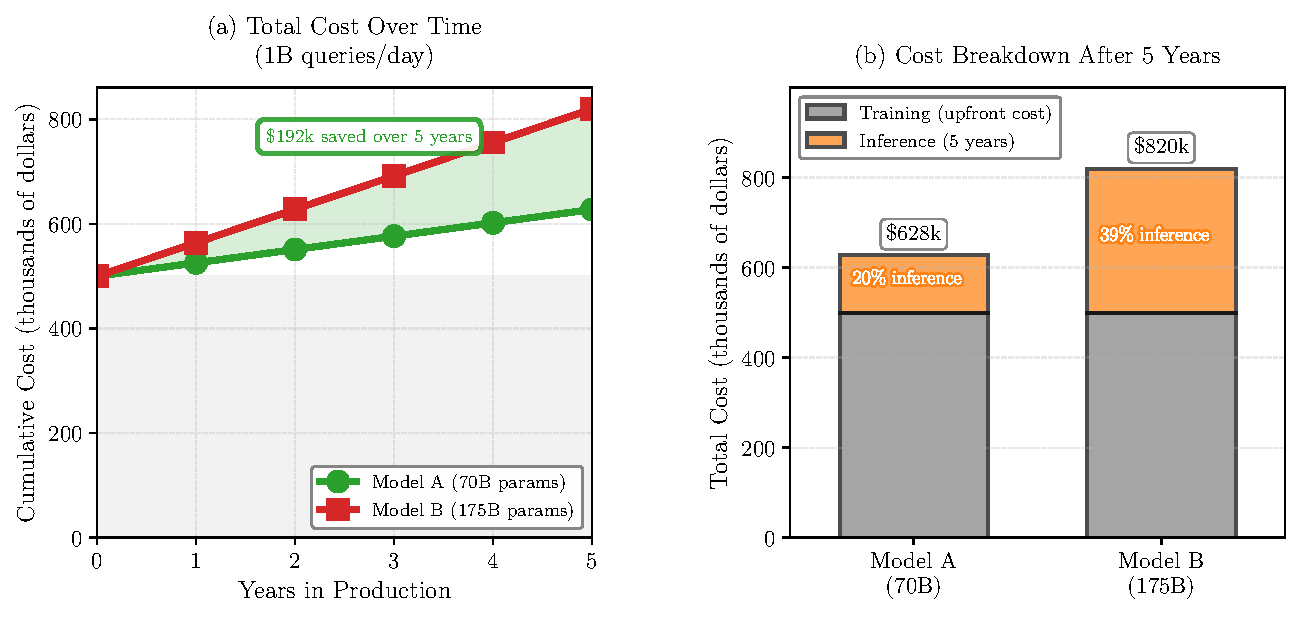
\includegraphics[width=\linewidth]{code/figures/ch12_uncertainty/fig_12_9_training_vs_inference_cost.pdf}
\caption{Total cost over a model's lifetime: training vs. inference. At high query volumes, inference can dominate; cost-optimal deployments favor smaller, data-rich models.}
\label{fig:training_vs_inference_cost}
\end{figure}


The decision framework is:

\begin{itemize}
\item \textbf{Low query volume} (< 1 million queries total): Training cost dominates. Use compute-optimal scaling without worrying about inference cost.

\item \textbf{Medium query volume} (1 to 100 million queries per year): Inference cost matters but is not dominant. Bias slightly toward smaller models if the performance loss is minor.

\item \textbf{High query volume} (> 100 million queries per year): Inference cost dominates. Optimize aggressively for inference efficiency, even if training costs double.
\end{itemize}

This analysis assumes you are serving in the cloud. If you are deploying on-device (e.g., in a mobile app), inference cost is not measured in dollars per query but in latency and battery life. The tradeoff tilts even more strongly toward smaller models because users will not tolerate slow or battery-draining models.

\vspace{1em}

\subsection{Data Quality Versus Data Quantity}

Scaling laws are often presented in terms of data quantity: train on more tokens to reduce loss. But not all tokens are equal. One million high-quality tokens can be worth more than 100 million noisy tokens. How do you think about this tradeoff?

From an information-theoretic perspective, data quality is about signal-to-noise ratio. High-quality data has high mutual information between inputs and outputs (for supervised learning) or between past and future tokens (for language modeling). Noisy data has lower mutual information because it includes patterns that do not generalize.

Let $S$ be signal tokens (high-quality) and $N$ be noise tokens (low-quality). The effective information content is not simply $S + N$ but something like $S + \alpha N$ where $\alpha < 1$ is the discount factor for noisy data. Empirically, $\alpha$ ranges from 0.1 to 0.5 depending on how noisy the data is.

This means that filtering and deduplication can improve model quality even when they reduce token count. If you filter out 50 percent of tokens but remove mostly noise, you have $0.5S + 0.05N$ instead of $S + 0.1N$, which could be better if noise tokens dominate.

The practical strategy is:

\begin{itemize}
\item \textbf{Deduplication:} Remove exact or near-duplicate documents. Duplicates inflate token count without adding information. They also cause memorization: the model overfits to duplicated content.

\item \textbf{Quality filtering:} Use heuristics (e.g., perplexity under a reference model, fraction of stop words, presence of structured data) or classifiers (train a model to predict whether text is high-quality) to score documents. Remove the bottom 10 to 30 percent by quality score.

\item \textbf{Domain balancing:} Oversample from high-quality domains (books, academic papers) and undersample from low-quality domains (forum posts, spam). This is a form of reweighting that increases effective information density.
\end{itemize}

The information-theoretic view is that noise increases $H(X)$ (the entropy of the data distribution) without decreasing $H(X|Z)$ (the conditional entropy given the true signal). This means the model wastes capacity learning patterns that do not reduce loss on clean data. By filtering noise, you reduce both $H(X)$ and $H(X|Z)$, improving the signal-to-noise ratio and making training more efficient.

\vspace{1em}

\subsection{Specialization Versus Generalization}

The final information budgeting question is when to specialize. You have a pretrained general-purpose model. Should you fine-tune it on domain-specific data, or should you train a new model from scratch on a mix of general and domain-specific data?

The tradeoff is between leveraging prior knowledge and avoiding interference. Fine-tuning starts from a good initialization, so it requires less compute and data to reach high performance on the domain. But if the domain is very different from the pretraining distribution, fine-tuning can hurt: the model's prior knowledge interferes with learning domain-specific patterns, a phenomenon called negative transfer.

Training from scratch avoids interference but requires more compute and data. You are learning both general language understanding and domain-specific knowledge simultaneously, which is redundant if the domain requires general understanding as a foundation.

The decision framework:

\begin{itemize}
\item \textbf{Fine-tune} when:
  \begin{itemize}
  \item The domain is similar to pretraining (e.g., medical text is similar to Wikipedia articles in structure, even if the vocabulary differs).
  \item You have limited domain-specific data (< 10B tokens).
  \item You need fast turnaround (fine-tuning takes hours to days, training from scratch takes weeks).
  \end{itemize}

\item \textbf{Train from scratch} when:
  \begin{itemize}
  \item The domain is very different from pretraining (e.g., programming code has different syntax and semantics than natural language).
  \item You have abundant domain-specific data (> 100B tokens).
  \item You can afford the compute and time for full training.
  \end{itemize}

\item \textbf{Continued pretraining} (a middle ground) when:
  \begin{itemize}
  \item You want to adapt a general model to a domain without catastrophic forgetting.
  \item Mix general and domain-specific data during fine-tuning to maintain broad capabilities while adding specialization.
  \end{itemize}
\end{itemize}

A worked example: suppose you want a medical language model. You have 50B tokens of medical text. A general-purpose 7B parameter model exists, pretrained on 2T tokens of web text. Should you fine-tune or train from scratch?

\textbf{Fine-tuning:} Start from the 7B model and fine-tune on 50B medical tokens. This requires $6 \times 7 \times 10^9 \times 50 \times 10^9 = 2.1 \times 10^{21}$ FLOPs, roughly 10,000 GPU-hours on A100s. The result will have good general language understanding plus medical specialization.

\textbf{Training from scratch:} Train a 3B parameter model on 50B medical tokens from random initialization. This requires $6 \times 3 \times 10^9 \times 50 \times 10^9 = 9 \times 10^{20}$ FLOPs, roughly 4,000 GPU-hours. The result will have strong medical specialization but weaker general understanding.

\textbf{Recommendation:} Fine-tune. The additional compute (10,000 vs 4,000 GPU-hours) buys you a larger model (7B vs 3B) with better general understanding. Unless your domain is extremely specialized and you never need to generalize beyond it, fine-tuning dominates.

\vspace{2em}

%==========================
\section{Synthesis and Exercises}
%==========================

Let's consolidate what we have learned and connect it back to the information-theoretic foundations from earlier chapters.

\vspace{1em}

\subsection{Scaling as Information Capacity Allocation}

Scaling is not just about bigger models. It is about allocating three scarce resources (parameters, data, and compute) to maximize information capacity under constraints.

\textbf{Parameters} give you memory capacity. They let you store patterns, facts, and transformations learned from data. But parameters have diminishing returns: the first billion parameters are more valuable than the tenth billion because they encode the most frequent patterns. This diminishing return manifests as the power law $L(N) \propto N^{-\beta}$.

\textbf{Data} gives you information content. More data means more examples of the patterns you want to compress, which improves your estimate of the true distribution. But data also has diminishing returns: later examples provide less new information because they are redundant with earlier examples. This manifests as $L(D) \propto D^{-\gamma}$.

\textbf{Compute} is the processing budget. It lets you match capacity to content by optimizing parameters on data. Compute has diminishing returns because optimization is subject to the law of diminishing marginal returns: the first gradient update moves you far, later updates move you less. This manifests as $L(C) \propto C^{-\alpha}$.

The optimal allocation balances these resources. Given compute budget $C$, the Chinchilla allocation $N^* \propto C^{0.5}$ and $D^* \propto C^{0.5}$ equalizes the marginal benefit of parameters and data. Spending more on one resource while starving the other leaves performance on the table.

This connects directly to the Minimum Description Length principle from Chapter 1 and Chapter 9. The model size $N$ is the description length of the model. The loss $L$ is the description length of the data given the model. The total description length is $\log N + n \cdot L$ where $n$ is the dataset size. Minimizing this total (for fixed $n$) gives you the compute-optimal tradeoff.

It also connects to PAC-Bayes from Chapter 9. The generalization bound has a term like $\sqrt{\mathrm{KL}(Q\,\|\,P)/n}$, where $\mathrm{KL}(Q\,\|\,P)$ grows with model complexity. Larger models typically imply larger KL (more information extracted from training), which requires more data $n$ to keep the bound tight. Scaling reflects this balance: as you scale compute, you grow both $N$ and $D$ so generalization does not collapse.

\vspace{1em}

\begin{pausebox}
\textbf{Reflecting on Scaling}

\vspace{0.5em}

Before moving to the exercises, reflect on how scaling connects to earlier chapters:

\vspace{0.5em}

From Chapter 1: Scaling laws are rate-distortion curves. Loss is distortion, compute is rate. The power law exponent encodes the intrinsic difficulty of compressing natural language.

\vspace{0.5em}

From Chapter 9: Scaling balances model complexity (KL divergence from prior) against fit (empirical risk). The Chinchilla allocation equalizes marginal benefit, just like PAC-Bayes suggests.

\vspace{0.5em}

From Chapter 11: Scaling informs information budgets. If you know the scaling law, you can predict the performance of different model-data combinations and choose the allocation that meets your constraints.

\vspace{0.5em}

Can you articulate why scaling laws follow power laws instead of exponentials or logarithms? Can you explain why emergent abilities appear at specific scales? Can you describe the tradeoff between training and inference costs?

\vspace{0.5em}

If these connections are clear, you are ready for the exercises. If anything feels uncertain, revisit the relevant section.
\end{pausebox}

\vspace{1.5em}

\subsection{Exercises}

\textbf{Exercise 1: Computing Chinchilla-Optimal Allocation}

You have a compute budget of $C = 5 \times 10^{22}$ FLOPs. Use the Chinchilla scaling law to compute the optimal model size $N_{\text{opt}}$ (in parameters) and dataset size $D_{\text{opt}}$ (in tokens). Define $C_{20} = C / 10^{20}$ and assume the empirical fit $N_{\text{opt}} \approx 0.73 \cdot C_{20}^{0.49}$ (in billions of parameters) and $D_{\text{opt}} \approx 22.8 \cdot C_{20}^{0.51}$ (in billions of tokens).

\vspace{0.5em}

\textbf{Exercise 2: Learning Rate Schedule Design}

You are training a 13B parameter model for 200,000 steps with a batch size of 2,048. Design a learning rate schedule with three phases: linear warmup over the first 1 percent of steps, constant learning rate for 80 percent of steps, and cosine decay for the final 19 percent of steps. Use a peak learning rate of $2 \times 10^{-4}$. Write the formula for the learning rate as a function of step $t$.

\vspace{0.5em}

\textbf{Exercise 3: Critical Batch Size Estimation}

You observe the following data from training runs at different batch sizes:

\begin{center}
\begin{tabular}{ccc}
Batch Size & Steps to Loss 2.5 & Wall-Clock Time \\
\hline
256 & 50,000 & 10 hours \\
512 & 26,000 & 6 hours \\
1,024 & 14,000 & 4 hours \\
2,048 & 8,000 & 3.5 hours \\
4,096 & 6,500 & 3.8 hours \\
8,192 & 6,000 & 4.5 hours \\
\end{tabular}
\end{center}

Estimate the critical batch size. Explain your reasoning.

\vspace{0.5em}

\textbf{Exercise 4: Training Versus Inference Cost Analysis}

You are deciding between two models for a chatbot application that will serve 10 million queries per day for two years. Model A has 10B parameters and achieves loss 2.4. Model B has 30B parameters and achieves loss 2.2. Training costs are \$200,000 for Model A and \$500,000 for Model B. Inference costs are \$1 per million parameters per billion queries. Which model has lower total cost over two years? At what query volume would the two models have equal total cost?

\vspace{0.5em}

\textbf{Exercise 5: Debugging Training Failure}

Your training loss curve looks like this:

\begin{itemize}
\item Steps 0-1,000: Loss decreases from 10.0 to 3.2
\item Steps 1,000-2,000: Loss decreases from 3.2 to 2.8
\item Steps 2,000-3,000: Loss oscillates between 2.6 and 3.1
\item Steps 3,000-4,000: Loss stays constant at 2.9
\end{itemize}

Gradient norms: Steps 0-2,000 average 0.3. Steps 2,000-4,000 average 0.05.

Diagnose the problem and propose a fix.

\vspace{0.5em}

\textbf{Exercise 6: Distributed Training Strategy}

You want to train a 150B parameter model. Each GPU has 80 GB of memory and can hold about 1.5B parameters (accounting for activations and optimizer states). You have access to 512 GPUs arranged in 64 nodes with 8 GPUs per node. Nodes have high-bandwidth interconnect (InfiniBand, 200 GB/s), but inter-node bandwidth is lower (Ethernet, 10 GB/s). Design a distributed training strategy using data parallelism, model parallelism, and/or pipeline parallelism. Justify your choices.

\vspace{0.5em}

\textbf{Exercise 7 (Hard): Deriving Power Law Exponent}

Using rate-distortion theory from Chapter 1, derive the power law exponent for the relationship between loss and parameters. Assume the data distribution is a Gaussian source with covariance structure that has eigenvalues decaying as $\lambda_k \propto k^{-\alpha}$ (this models power-law decay in natural language). The model has $N$ parameters. Show that $L(N) \propto N^{-\beta}$ and compute $\beta$ in terms of $\alpha$.

\vspace{0.5em}

\textbf{Exercise 8 (Hard): Designing a Scaling Experiment}

You have trained models at three scales: 100M, 1B, and 10B parameters, each with compute-optimal data. The losses are 3.2, 2.6, and 2.1 respectively. You want to predict the loss of a 100B parameter model trained with compute-optimal data. Fit a power law to the existing data points and extrapolate to 100B. Estimate the compute budget required. What assumptions are you making? How could you validate your prediction before committing to the full training run?

\vspace{1.5em}

This chapter has explored the empirical regularities that govern how model performance scales with resources, the practical dynamics of training large models, and the information-theoretic framework for making allocation decisions. We saw that scaling laws are not accidents but emerge from fundamental principles of compression and rate-distortion theory. We learned how to navigate training challenges like learning rate schedules, batch size selection, stability issues, and distributed training. And we developed an information budget framework for deciding when to scale, how to allocate compute between training and inference, and when to specialize through fine-tuning.

In the next chapter, we will turn to production systems: deploying models reliably under real-world constraints. Scaling improves raw performance, but deployment adds new constraints like latency, cost, and failure handling. The information-theoretic tools we have built will help us reason about these tradeoffs and design systems that hold up in practice.

\vspace{1em}

\begin{pausebox}
\textbf{Key Takeaways from Chapter 12}

Scaling laws describe power-law relationships between loss and resources (compute, parameters, data). These laws are not arbitrary; they emerge from rate-distortion theory and the diminishing returns of compression. The Chinchilla discovery showed that compute-optimal training balances parameters and data: both should scale as $\sqrt{C}$. Training dynamics require careful management of learning rates, batch sizes, and stability. Learning rate schedules use warmup, stable training, and decay. Batch size tradeoffs balance exploration and efficiency, with a critical size beyond which gains plateau. Stability requires gradient clipping, NaN detection, and checkpoint recovery. Distributed training splits work across GPUs using data, model, or pipeline parallelism depending on model size. Information budgeting means allocating compute between training and inference, prioritizing data quality over quantity, and choosing between fine-tuning and training from scratch based on domain similarity. Scaling is ultimately about allocating information capacity efficiently under constraints.
\end{pausebox}
